\question{
    平行板电容器内有两层介质,它们的厚度分别为$l_1$和$l_2$,电容率为$\eps_1$和$\eps_2$,今在两板上接上电动势为$\huae$的电池,求
}

\subquestion{电容器两板上的自由电荷面密度$\wf{}$;}

\subquestion{介质分界面上的自由电荷面密度$\wf{}$. }

\subquestion{若介质是漏电的,电导率分别为$\sig_1$和$\sig_2$,当电流达到恒定时,上述两问的结果如何?}

\begin{figure}[h]
    \centering
    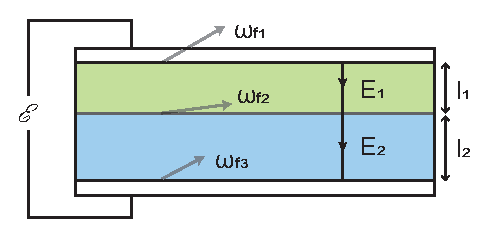
\includegraphics[width=8cm]{img/1.2/电容器.eps}
    \caption{平行板内有两层介质(示意图)}
    \label{1.2_fig:电容器}
\end{figure}

如图\ref{1.2_fig:电容器},考虑无边缘效应的理想电容器和均匀介质,设电容器上极板与上层介质之间的自由电荷面密度为$\wf{1}$,两层介质之间的自由电荷面密度为$\wf{2}$,电容器下极板与下层介质之间的自由电荷面密度为$\wf{3}$,两层介质内的电场强度大小为$E_1$和$E_2$,方向如图。

有静电场边值关系
\begin{equation}
    \begin{bmatrix}
    1  & 0\\
    -1 & 1\\
    0  & -1
    \end{bmatrix}
    \begin{bmatrix}
    \eps_1 E_1\\
    \eps_2 E_2
    \end{bmatrix}
    =
    \begin{bmatrix}
    \wf{1}\\
    \wf{2}\\
    \wf{3}
    \end{bmatrix},
    \label{1.2_边值关系}
\end{equation}
电势边界条件
\begin{equation}
    \huae = E_1 l_1 + E_2 l_2. \label{1.2_电势条件}
\end{equation}
仅凭(\ref{1.2_边值关系})(\ref{1.2_电势条件})并不足以同时确定$\wf{1}$、$\wf{2}$、$\wf{3}$。这是因为对于这样一个没有其他约束(诸如恒定电流条件)的静电场系统,两介质之间的界面仍然有一个可以自由选取的边界条件(上下极板的边界条件由电势条件给出)。也就是说,我们对于绝缘的介质而言,两介质之间的$\wf{2}$是一个待定的值,对于任何一个可能的$\wf{2}$取值,我们可以解出对应的不同的$\wf{1}$、$\wf{3}$(这类似于静力学中的超静定问题)。从题目的表述中,我们并不能找到$\wf{2}$取何值的依据,因此我们需要根据一般情况设定一个$\wf{2}$取值,这是必要的,后文我会由叠加原理和唯一性定理给出一个严谨的证明。现在我们不妨取
\begin{equation}
    \wf{2} = 0. \label{1.2_w2}
\end{equation}
由(\ref{1.2_边值关系})(\ref{1.2_电势条件})(\ref{1.2_w2})解得
\begin{eqnarray}
    \wf{1} &=& \frac{\huae}{{l_1}/{\eps_1}+{l_2}/{\eps_2}}, \label{1.2_w1} \\
    \wf{3} &=& - \frac{\huae}{{l_1}/{\eps_1}+{l_2}/{\eps_2}}.  \label{1.2_w3}
\end{eqnarray}

下面我们证明(\ref{1.2_w2})的存在是必要的。我们考虑反证法:假设我们认为给定上下极板的电势(\ref{1.2_电势条件})即是给出了完备的边界条件,那么不需要(\ref{1.2_w2})就可以解出唯一的$\wf{2}$、$E_1$、$E_2$,这是由唯一性定理保证的。我们取(\ref{1.2_w2})为试探解,显然可以得到满足边界条件(\ref{1.2_电势条件})的解(\ref{1.2_w3})(\ref{1.2_w3}),并且解出电场强度大小
\begin{eqnarray}
    E_1 &=& \frac{\huae/\eps_1}{{l_1}/{\eps_1}+{l_2}/{\eps_2}}, \label{1.2_E1} \\
    E_2 &=& \frac{\huae/\eps_2}{{l_1}/{\eps_1}+{l_2}/{\eps_2}}.  \label{1.2_E2}
\end{eqnarray}
这应当是(\ref{1.2_电势条件})下的唯一解。现在我们考虑另一个试探解
\begin{equation}
    \wf{2}'=\wf{2}+\Delta\wf{2}.
\end{equation}
根据叠加原理,将现在的系统考虑为原系统和新系统($\huae=0$,$\wf{2}=\Delta\wf{2}\ne0$)的线性叠加,容易得解
\begin{eqnarray}
    E_1' &=& \frac{\huae/\eps_1}{{l_1}/{\eps_1}+{l_2}/{\eps_2}} - \frac{\Delta\wf{2} l_2}{\eps_1 l_2 + \eps_2 l_1} , \label{1.2_E1'} \\
    E_2' &=& \frac{\huae/\eps_2}{{l_1}/{\eps_1}+{l_2}/{\eps_2}} + \frac{\Delta\wf{2} l_1}{\eps_1 l_2 + \eps_2 l_1} .  \label{1.2_E2'}
\end{eqnarray}
此为异于(\ref{1.2_E1})(\ref{1.2_E2})的可行解,与静电场的唯一性定理矛盾,故假设不成立,证明(\ref{1.2_w2})的存在是必要的。

基于上述分析,我们还可以写出该系统的通解
\begin{eqnarray}
    \wf{1} &=& \frac{\huae}{{l_1}/{\eps_1}+{l_2}/{\eps_2}} - \frac{\eps_1/l_1}{\eps_1/l_1 + \eps_2/l_2}\wf{2}, \\
    \wf{2} &=& \mathrm{arbitrary~constant}, \\
    \wf{3} &=& - \frac{\huae}{{l_1}/{\eps_1}+{l_2}/{\eps_2}} - \frac{\eps_2/l_2}{\eps_1/l_1 + \eps_2/l_2}\wf{2}. 
\end{eqnarray}

若介质是漏电的,在稳恒电流情况下我们由电荷守恒得到约束关系
\begin{equation}
    - \sig_1 E_1 + \sig_2 E_2 = 0. \label{1.2_电荷守恒}
\end{equation}
由(\ref{1.2_边值关系})(\ref{1.2_电势条件})(\ref{1.2_电荷守恒})得解
\begin{eqnarray}
    \wf{1} &=& \frac{\sig_2\eps_1\huae}{\sig_1l_2+\sig_2l_1}, \\
    \wf{2} &=& \frac{(\sig_1\eps_2-\sig_2\eps_1)\huae}{\sig_1l_2+\sig_2l_1}, \\
    \wf{3} &=& -\frac{\sig_1\eps_2\huae}{\sig_1l_2+\sig_2l_1}. 
\end{eqnarray}
